%-----------------------------------------------------------------------------
%
%               Template for sigplanconf LaTeX Class
%
% Name:         sigplanconf-template.tex
%
% Purpose:      A template for sigplanconf.cls, which is a LaTeX 2e class
%               file for SIGPLAN conference proceedings.
%
% Guide:        Refer to "Author's Guide to the ACM SIGPLAN Class,"
%               sigplanconf-guide.pdf
%
% Author:       Paul C. Anagnostopoulos
%               Windfall Software
%               978 371-2316
%               paul@windfall.com
%
% Created:      15 February 2005
%
%-----------------------------------------------------------------------------


\documentclass{sigplanconf}

% The following \documentclass options may be useful:

% preprint      Remove this option only once the paper is in final form.
% 10pt          To set in 10-point type instead of 9-point.
% 11pt          To set in 11-point type instead of 9-point.
% authoryear    To obtain author/year citation style instead of numeric.

\usepackage{amsmath}
\usepackage{epsfig}
\usepackage{alltt}
\usepackage{times}
\usepackage{array}
\usepackage{graphicx}



\begin{document}

\special{papersize=8.5in,11in}
\setlength{\pdfpageheight}{\paperheight}
\setlength{\pdfpagewidth}{\paperwidth}

\conferenceinfo{CONF 'yy}{Month d--d, 20yy, City, ST, Country} 
\copyrightyear{20yy} 
\copyrightdata{978-1-nnnn-nnnn-n/yy/mm} 
\doi{nnnnnnn.nnnnnnn}

% Uncomment one of the following two, if you are not going for the 
% traditional copyright transfer agreement.

%\exclusivelicense                % ACM gets exclusive license to publish, 
                                  % you retain copyright

%\permissiontopublish             % ACM gets nonexclusive license to publish
                                  % (paid open-access papers, 
                                  % short abstracts)

\titlebanner{banner above paper title}        % These are ignored unless
\preprintfooter{short description of paper}   % 'preprint' option specified.

\title{Power Aware HTTP: Modifying HTTP to optimize power consumption}


\authorinfo{Ankit Goyal}
{University of Texas at Austin}
           {ankit@cs.utexas.edu}
\authorinfo{Sreedevi Surendran}
{University of Texas at Austin}
           {sreedevi@cs.utexas.edu}

\maketitle

\begin{abstract}
\noindent A major part of the Internet works on the HTTP protocol. Optimizations to the protocol have been suggested to improve the performance of the protocol. However, less attention has been paid to the power consumption aspect of the protocol which is bound to play a significant role in the coming years due to an increase in mobile devices which are constrained by limited power capabilities. In this paper, we first analyze where exactly the power is consumed, how configuration changes affect power consumption and then we propose a noval solution to reduce the power consumed by HTTP without compromising on performance. 

\end{abstract}

% general terms are not compulsory anymore, 
% you may leave them out

\keywords
Network Protocol, HTTP, TCP, Power Aware, Wireless Networking

\section{Introduction}

The field of wireless communication has seen tremendous progress in recent years. Mobile devices are on the increase and being connected to the internet while on the move is essential in today’s society. One of the greatest constraints to realizing this goal is finite power supply which leads to short continuous operation time of mobile devices.

In this context, we first try to pinpoint the part of the HTTP protocol which leads to power consumption. We then make changes to the configurable server side properties including timeout, keepalive values etc. to analyze the level of impact these parameters have on the power consumption and finally, propose a power aware HTTP protocol that can optimize the power consumption of HTTP.

The rest of this paper is organized as follows: Section 2 highlights the background and related works of hypertext transfer protocol, transmission control protocol and power consumption issues over HTTP. Section 3 highlights the motivation behind this paper. Section 4 presents our proposed implementation of a power aware HTTP. Section 5 outlines the challenges faced during the course of the implementation. Section 6 outlines the results of our implementaion. Section 7 lists some other optimizations to optimize the power consumption of HTTP. Section 8 discusses related works. Section 9 includes our concluding remarks. Section 10 discusses the future work in the context of power optimziation of HTTP. Section 11 lists the references.

\section{Background}

In this section we give a brief overview of the HTTP protocol. This is followed by an overview of the connection establishment and teardown in TCP. We then discuss the inefficiencies in the HTTP protocol as it is implemented today and the power consumption observed in HTTP.

\subsection{HTTP Protocol Overview}

The HTTP protocol follows a client server model where a request (in simple ASCII format) is sent from the client to the server, followed by a response (in simple ASCII format) sent from the server to the client. An HTTP request includes the following elements: a method which can be either GET, PUT, POST, DELETE etc; a set of headers which specifies the type of content the client is ready to accept, authentication data etc; a payload field to hold data for PUT method etc. The server processes the request and sends a response to the client. The response includes a status code that indicates whether the request was successful or not and if not, the errors in the request are returned. The response also includes information about the data returned by the server like content-length of the response and the output generated by the server-side script (can be an HTML/ XML/JSON file etc). 

HTTP utilizes TCP for reliable transfer of information over the internet. To analyze the power consumption model of HTTP, it is relevant to give a brief overview of the TCP connection establishment and teardown.



\subsection{TCP Protocol Overview}
\subsubsection{Connection Establishment}
For a client to establish a TCP connection with a server, the client must send a SYN and receive an ACK for it from the server. Thus, conceptually, there should be four control messages passed between the devices. However, it's inefficient to send a SYN and an ACK in separate messages when one could communicate both simultaneously. Thus, in the normal sequence of events in connection establishment, one of the SYNs and one of the ACKs is sent together by setting both of the relevant bits (a message sometimes called a SYN+ACK). This makes a total of three messages, and is called a three-way handshake.

\subsubsection{Connection Teardown}
Each side terminates its end of the connection by sending a special message with the FIN (finish) bit set. This message, sometimes called a FIN, serves as a connection termination request to the other device, while also possibly carrying data like a regular segment. The device receiving the FIN responds with an acknowledgment to the FIN to indicate that it was received. The connection as a whole is not considered terminated until both sides have finished the shut down procedure by sending a FIN and receiving an ACK.
Thus, termination isn't a three-way handshake like establishment: it is a pair of two-way handshakes. The states that the two devices in the connection move through during a normal connection shutdown are different because the device initiating the shutdown must behave differently than the one that receives the termination request. In particular, the TCP on the device receiving the initial termination request must inform its application process and wait for a signal that the process is ready to proceed. The initiating device doesn't need to do this, since the application is what started the ball rolling in the first place.

\subsection{Inefficiencies of HTTP}
The HTTP protocol as it is implemented today has some notable inefficiencies. According to the current specification, while fetching a webpage using HTTP, explicit calls to the server are required to fetch individual resources on a webpage even though both client and server know that multiple resources need to be shared. In HTTP/1.0, a new conenction is established on every subsequent request(Every such call requires the setup of a new TCP connection.). This increase in the number of calls to the server adds to the power consumption and latency. However this was changed in the specification of HTTP/1.1. Modern browsers try to  optimize this problem by maintaining "persistent" connections and pipelining requests. Also, HTTP does not  impose any requirements on data compression. 


\subsection{Power Consumption in HTTP}

\subsubsection{ Non Persistent HTTP Connections}

In non-persistent HTTP connections, all the resources on a web page are fetched using different TCP connection. Since the client sets up a new TCP connection for every HTTP request number of requests are propotional to the number of resources on the page. A typical web page consists of lot of images and text, and all the resources are fetched using a different HTTP connection which increases the number of round trips. Each round trip requires allocation of new resources such as port numbers, bookkeeping data structures, etc. which leads to more processing power. Figure 1 shows the establishment of a new TCP connection to fetch each resource on a webpage.

Due to an increase in the effective number of requests the probability of collisions increase and TCP’s congestion response by slow start approach [2] leads to inefficient use of  the available network bandwidth. TCP does not reach full throughput until the effective congestion window size is at least the product of the round-trip delay and the available network bandwidth [1]. This means that slow start limits TCP throughput, which leads to more roundtrips and consequently higher power consumption.

\begin{figure}[ht!]
\centering
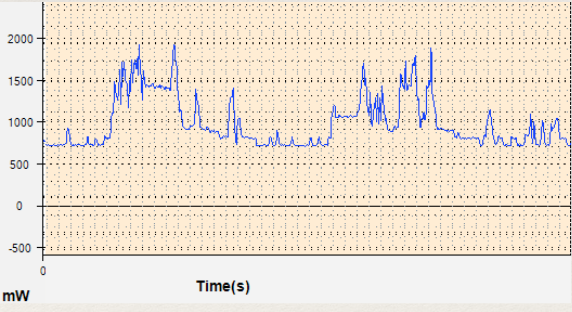
\includegraphics[width=80mm]{powerconsumption2.png}
\caption{Non-Persistent HTTP Connection on 802.11}
\label{fig:sp_gd_mnist}
\end{figure}




\begin{figure}[ht!]
\centering
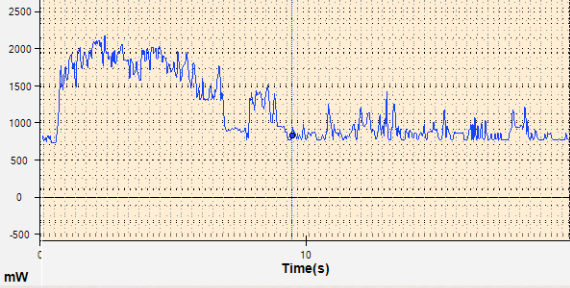
\includegraphics[width=80mm]{powerconsumption1.png}
\caption{Persistent HTTP Connection on 802.11 }
\label{fig:sp_gd_mnist}
\end{figure}


\subsubsection{Persistent HTTP Connections}

In a persistent HTTP connection, a single TCP connection is used to send and receive multiple web requests using the keep-alive header field. which eliminates the need of establishment of new TCP connection to fetch each resource. This reduces the number of effective calls. As corroborated by our experiments power consumption is directly propotional to the number of requests made. Figure 2 shows that all the resources are fetched using a single TCP connection. On 802.11, comparing the average energy consumed by non-persistant connection we found it to be 11.8\% more than that consumed by persistent connections.

However in practice each server has a limit on number of concurrent HTTP connections it can keep, we need to find an optimal time period to keep the TCP connection open given variables like content-length of the data being exchanged. Moreover keeping connections open on a cellular network may not be the most optimcal strategy since a client (unnecessarily) remains in a high power consumption state during that period as seen in Figure 3. 

\section{Motivation}
The effect of an increase in the number of calls to the server is more severe in resource-constrained devices. Since the power consumption increases with the number of requests made, we focus on novel methods to reduce the number of HTTP requests made by a webpage.

Today, websites try to reduce latency and power consumption by caching various resources. However, client need to check with the server about the freshness of the resources. Typically conditional HTTP enabled by {\it If-Modified-Since} and {\it If-None-Match} header fields are used by clients to check the validity of cache; where resource is returned only if it has been changed on the server otherwise a status code of 304 (not modified) in response will be returned without any message-body. 

In HTTP/1.1, to load a cached webpage, the number of conditional GET requests equals the number of resources. For resources that are not modified often, this is an unnecessary overhead.

Table 1. shows the number of unmodified resources relative to the total requests made by the 10 most popular websites based on the study by Alexa Internet (which ranks webistes based on page views and unique site users.)
It can be seen that a majority of the resources on most of these cached webpages were seldom modified and unnecessary HTTP calls are being made to server to check the freshness of resources.

\begin{table}[htbp]
\centering
\caption{}
\begin{tabular}{|c|c|c|}
\hline
 & \multicolumn{1}{l|}{Total Requests} & \multicolumn{1}{l|}{Not Modified} \\ \hline
Google & 21 & 18 \\ \hline
Apple & 83 & 81 \\ \hline
Facebook & 24 & 20 \\ \hline
Youtube & 21 & 8 \\ \hline
Yahoo & 98 & 39 \\ \hline
Baidu & 13 & 10 \\ \hline
Wikipedia & 33 & 33 \\ \hline
Twitter & 5 & 3 \\ \hline
Tencent QQ & 201 & 69 \\ \hline
Amazon & 215 & 190 \\ \hline
\end{tabular}
\label{}
\end{table}

\section{Proposal}

In pratice majority of resources on a website change infrequently and we try to reduce the number of conditional requests required to check whether the resource has been modified or not. For a page that is loaded from the cache, we propose \it{Power-Aware HTTP} \rm  a noval extension to HTTP which involves the addition of two new header fields to the HTTP GET request method - \bf{check-resource} \rm and \bf{resource-status} \rm. These headers will enable a client to check the status of multiple resource in a single web request.  

As shown in Figure 3., the header \it{check-resource} \rm header will allow a client to pass MD5 hash values for multiple resources and \it{resource-status} \rm will allow the server to send the validity information for multiple resources. Basically when a cached webpage is to be loaded, a single GET request will be made which will contain the MD5 hash of all the resources on the page. The server uses MD5 hash to match resources and checks whether the resources have been modified (one-by-one) and returns the status (modified/not modified) for every resource to the client. The client then makes GET requests for only the resources that have been modified.


\begin{figure}[ht!]
\centering
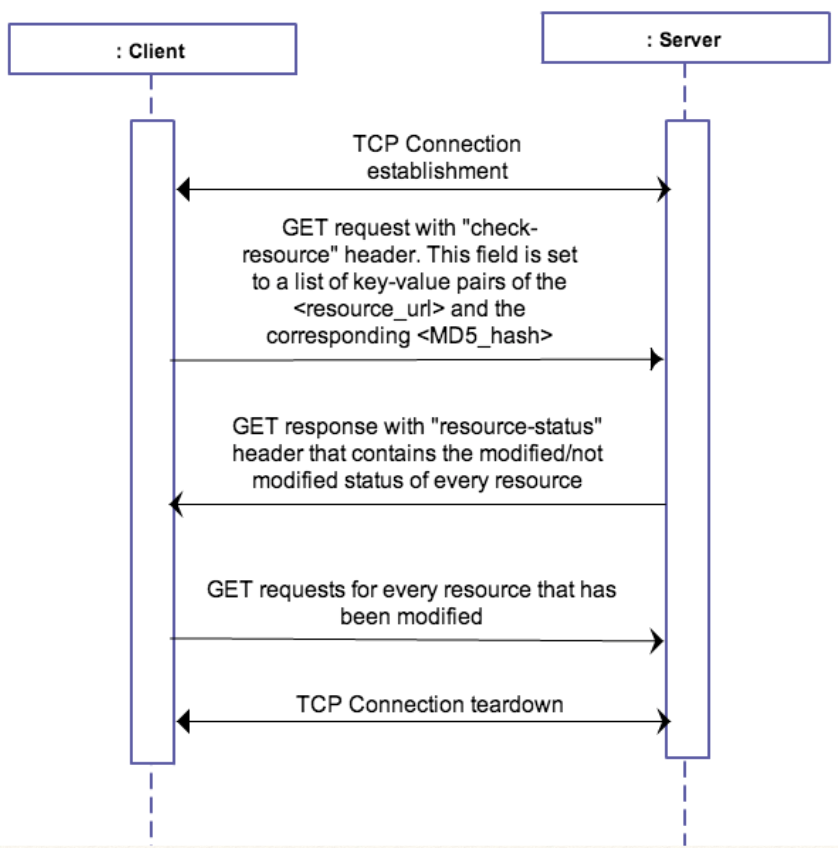
\includegraphics[width=80mm]{proposal}
\caption{Client-Server interaction using Power-Aware HTTP }
\label{fig:sp_gd_mnist}
\end{figure}



\section{Implementation}

We implemented our proposal at the application layer, and tested its performance over wifi and cellular network (3G).

\subsection{Client}

An additional header field {\it check-resource} is added to the single GET request made by the client. 
The value of this field will be set to a list of key-value pairs of the resource-url and the corresponding MD5 hash.  When the client receives the modified/not modified status of the individual resources from the server's response header, it will then make GET requests for only those resources that have not been modified.

We implemented a native android application (shown in figure 4.) that allowed us to make a request for multiple resources with the new header, \it{check-resource} \rm. 


\subsection{Server}

The server responds with an additional response header {\it resource-status} which is a bitmap containing the modified/not modified status of every resource on the webpage. 

We used ruby framework caleld Sinatra, which allowed us to add the middleware to intercept the conditinal request and add a new header field to the response header of Web-brick server.

\subsection{Technical Setup}
The components used for the implementation are listed below.

\subsubsection{Hardware}

\noindent1. Power Monitor by Monsoon Solutions. \newline
2. Mobile Device: HTC desire one running Android 4.2.2 

\subsubsection{Software}

1. Application: Native android application

2. Servers: Apache Tomcat, Web-brick

3. Framework: Sinatra

4. Analysis: Matlab

\begin{figure}[ht!]
\centering
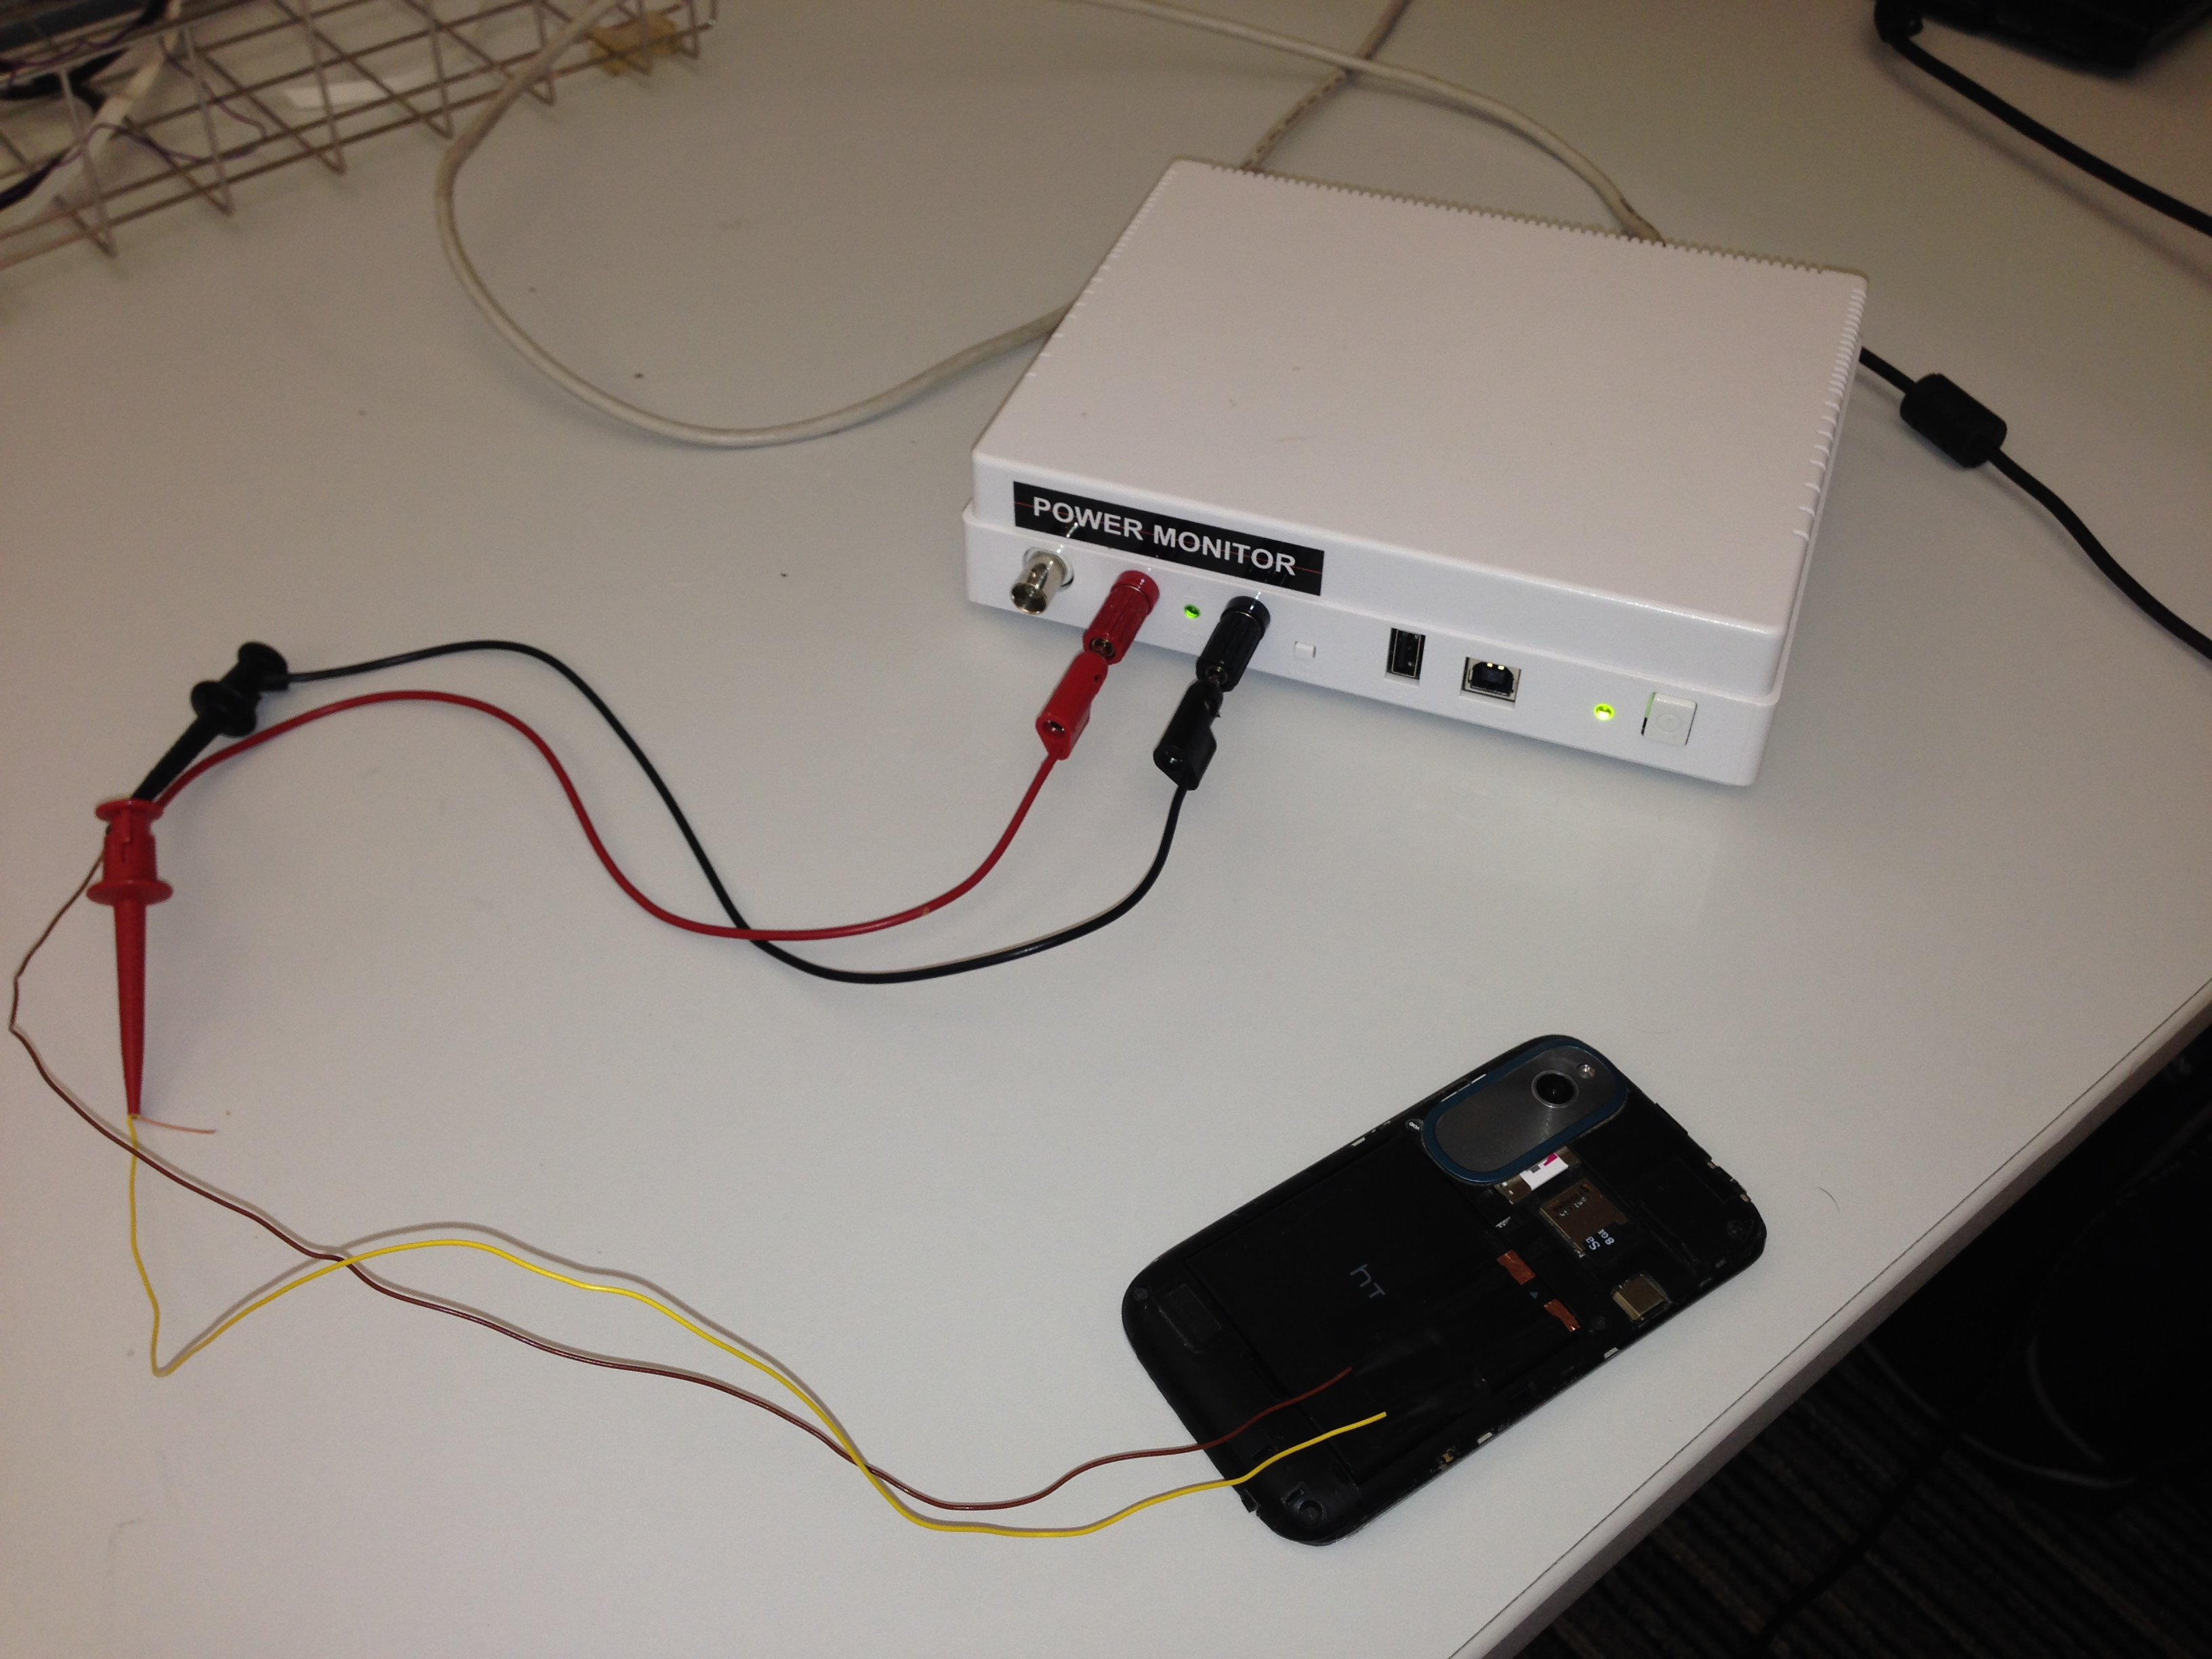
\includegraphics[width=70mm]{monitor.jpg}
\caption{Monsoon Solutions’ Power Monitor and PowerTool software were used to capture power measurements for HTTP interactions on the Android device. }
\label{fig:sp_gd_mnist}
\end{figure}



\section{ Challenges}

While measuring power for different HTTP requests, a lot of spikes were observed in the power consumption graph which were not related to HTTP, since the connection was either in an idle state or the HTTP request had been completed. These could have happened due to the following reasons: \\
a) Different browsers have different power consumptions and have different scheduling policy to fetch the results. For example, Google Chrome starts fetching a page as soon as you start typing the URL which may require additional processing and thus add to the power consumption.
\it{Solution:} \rm To address this, we created an Android app that allowed us to make HTTP calls with custom headers for various scenarios eliminating any power consumption due to rendering or other optimizations. All the HTTP connections were reused and the persistence of a connection was controlled from the server side by setting the KeepAlive flags.

b) There are lot of background processes in an Android device that consume power and it becomes difficult to know whether the power spikes are due to the monitored HTTP calls or due to other processes in the system.
\it{Solution:} \rm To alleviate the effect of other applications, we considered the average power consumption over several readings. We also subtracted the baseline from the original signal to mitigate the effects of continuously running background processes. We applied the Butterworth low-pass filter to mitigate the interference of high frequency noise.


\section{Results}
We evaluated the performance of Regular HTTP and Power-Aware HTTP over 802.11 and Cellular network for different number of modified resources.  

\subsection{Power consumption in Cellular}
Table 2. shows the average energy consumed by both Power-Aware HTTP and Regular HTTP over a cellular network for different number of modified resources. It can be seen from Figure 5, that the Power-Aware HTTP consumes much less power than the Regular HTTP in case the number of modified resources are less. Our solution performs worse than Regular HTTP only in case when all the resources are modified, but in a typical webpage this is not a common scenario as seen in Table 1. In our experiments we observed an average improvement of 112.3\% in power consumption assuming probability of a resource being modified to be 1/2 for all the 10 resources we tested for.

\begin{table}[htbp]
\centering
\caption{Power consumption in mJ for different HTTP implementations.}
\begin{tabular}{|r|r|r|r|}
\hline
\multicolumn{1}{|l|}{} & \multicolumn{1}{l|}{Power-Aware HTTP} & \multicolumn{1}{l|}{Regular HTTP} & \multicolumn{1}{l|}{Difference} \\ \hline
0 & 8813.55 & 5109.29 & 3704.26 \\ \hline
1 & 22819.33 & 7077.08 & 15742.25 \\ \hline
4 & 26546.05 & 10279.8 & 16266.25 \\ \hline
6 & 32878.45 & 15107.92 & 17770.53 \\ \hline
10 & 50532.2 & 55641.49 & -5109.29 \\ \hline
\end{tabular}
\label{}
\end{table}



\begin{figure}[ht!]
\centering
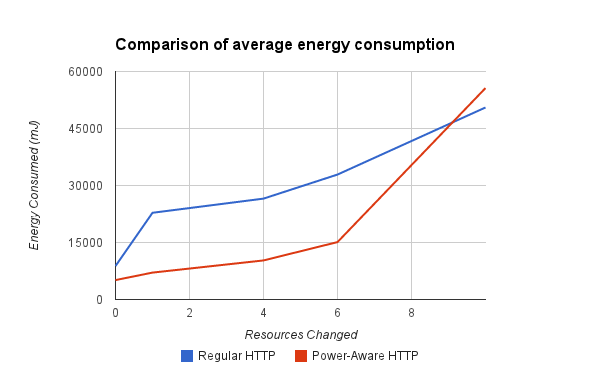
\includegraphics[width=80mm]{avg_energy_cell.png}
\caption{Comparison of energy consumption in a cellular network}
\label{fig:sp_gd_mnist}
\end{figure}

\subsection{Power consumption in 802.11}
Table 3. shows the average energy consumed by both Power-Aware HTTP and Regular HTTP over 802.11 for different number of modified resources. It can be seen from Figure 6, that the Power-Aware HTTP consumes marginally less power than the Regular HTTP in case the number of modified resources are less. The actual power consumption may be less or more depending on the network conditions but our solution will always perform better(except the worst case) since the number of requests made are less. Again assuming the probability of a resource being modified to be 1/2 our solution showed an improvement in power consumption by 12.4\%.


Note that the relative improvement of Power-Aware HTTP is significantly less in 802.11 than the cellular network since in cellular the radio stays in high power mode for the duration during which the transfer is taking place as shown in Figure 7. 802.11 is much more power efficient than the cellular and it can be seen in Figure 8. that the power consumption during the ideal period goes down in case of 802.11


\begin{table}[htbp]
\centering
\caption{Power consumption in wifi}
\begin{tabular}{|r|r|r|r|}
\hline
\multicolumn{1}{|l|}{} & \multicolumn{1}{l|}{Regular HTTP} & \multicolumn{1}{l|}{Power-Aware HTTP} & \multicolumn{1}{l|}{Difference} \\ \hline
0 & 402.68 & 452 & 49.32 \\ \hline
2 & 418.32 & 533.68 & 115.36 \\ \hline
5 & 480 & 544.56 & 64.56 \\ \hline
8 & 680.54 & 758.05 & 77.51 \\ \hline
10 & 809.23 & 791.13 & -18.1 \\ \hline
\end{tabular}
\label{}
\end{table}

\begin{figure}[ht!]
\centering
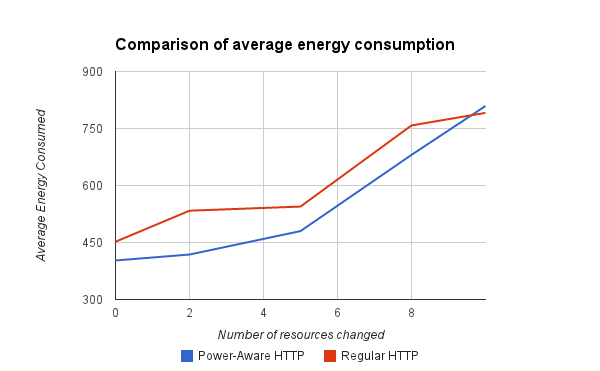
\includegraphics[width=80mm]{avg_energy_wifi.png}
\caption{Comparison of energy consumption in 802.11}
\label{fig:sp_gd_mnist}
\end{figure}




\subsection{Best Case}

In this more likely case, for a cached webpage with n resources, out of which m (m \textless \textless n) resources have been modified: regular HTTP makes {\it n} GET requests. Power-aware HTTP, on the other hand, makes {\it (1+m)} GET requests.



\subsection{Worst Case}

For a cached webpage with n resources, out of which all n resources have been modified, regular HTTP
makes {\it n} GET requests whle power-aware HTTP makes {\it (1+n)} GET requests.



\begin{figure}[ht!]
\centering
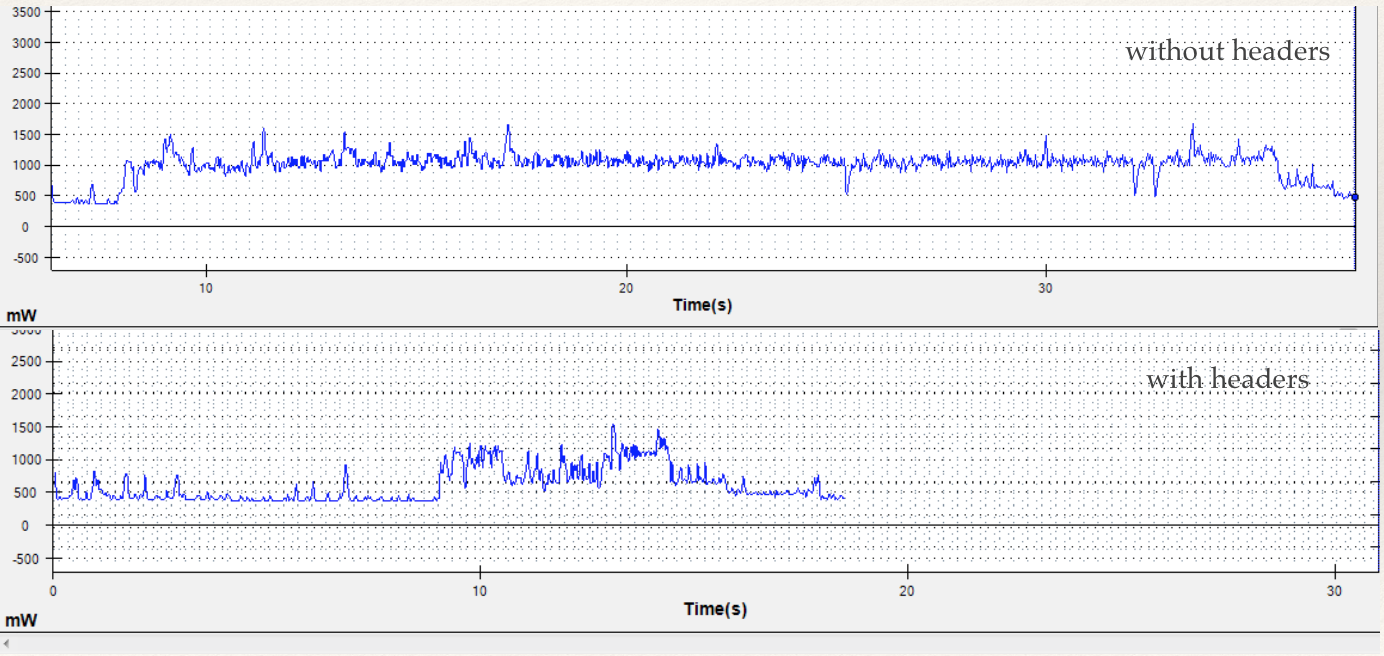
\includegraphics[width=80mm]{Cellular_combined.png}
\caption{Power consumption pattern in Cellular network }
\label{fig:sp_gd_mnist}
\end{figure}

\begin{figure}[ht!]	
\centering
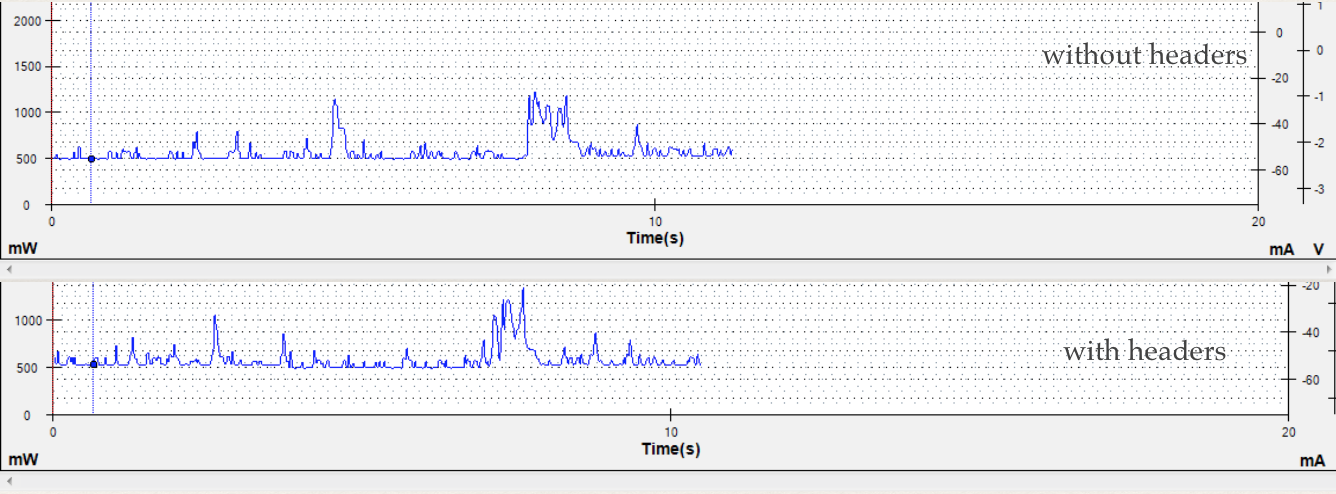
\includegraphics[width=80mm]{Wifi_combined.png}
\caption{Power consumption pattern in 802.11}
\label{fig:sp_gd_mnist}
\end{figure}



\section{More Optimizations}

We looked at some of the optimizations made by modern browsers. One of the optimizations done by Google Chrome to reduce latency is pre-fetching the URL before a user actually finishes typing the URL.
 
Server logs in the figure 9. shows that as soon as user starts typing, Chrome starts making HTTP requests for each typed character. This approach reduces latency but consumes a lot of power and wastes a lot of network resources. 

Solution: We try to address this problem by making server give hint to client to prevent premature fetching of urls by modifying the response of 404. We return the possible URL options matching the pattern in an additional header field. In case of cellular network, we found that the energy consumption was less by 15.8\%.




\begin{figure}[ht!]
\centering
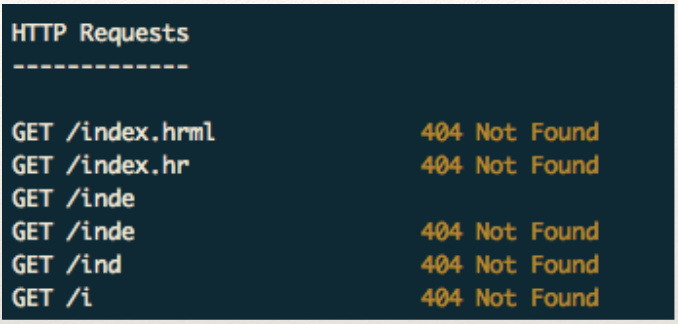
\includegraphics[width=80mm]{chrome}
\caption{Chrome URL Pre-Fetch}
\label{fig:sp_gd_mnist}
\end{figure}



\section{ Related Works}

Other works that have tried to address the inefficiencies of HTTP include the work on improving HTTP latency by 22\% [1]. The authors propose two new HTTP request methods: GETALL and GETLIST to retrieve all the resources on a webpage with a single call. Authors in [1] doesn't consider the case when the webpage is cached and  we propose to have a cient query the server to check the resource change status and make subsequent GET requests for the modified resources based on the response from the server.

Another work suggests the use of a web proxy to reduce power consumption by not waiting for requests on a WAN and the use of request pipelining to reduce the wait period [2].

\section{Conclusions}

Power consumption in a resource-constrained device depends on a number of factors. In our approach, we have targeted novel means to reduce the number of HTTP requests. In the implentation of HTTP today, all the resources on a cached webpage are fetched using different HTTP connections which increases the number of round trips. We propose an extension to HTTP to reduce the number of requests. The proposed solution shows clear quantitative gains in reducing power consumption over the existing implementation of HTTP. 

Our solution to have the server provide hints to the client to handle the pre-fetch url problem may not be the most optimal solution but we try to show that HTTP needs to be smart enough 	to accomodate optimizations aimed at improving performane.

Standardization is necessary for the solution to work accross all browsers. The proposed solution cannot be used until all browsers provide the fucntionality to an HTTP GET request with the {\it check-reosurce} header. Different hosting services can provide this functionality if a standard is established.

\section{Future Work}

More robust analysis of the performance by taking power measurement readings over a period of normal usage. It would be interesting to see the performance on the desktop PCs since the work is equally applicable on all devices. 

\acks

Thank you to Lili



\bibliographystyle{abbrvnat}
% The bibliography should be embedded for final submission.

\begin{thebibliography}{}
\softraggedright

\bibitem[Venkata N. Padmanabhan. et~al.(1995) Venkata N. Padmanabhan ]{latency1}
 Venkata N. Padmanabhan and Jeffrey C. Mogul ,Improving HTTP Latency. Computer Networks and ISDN Systems.

\bibitem[Van Jacobson. et~al.(1998)  Van Jacobson]{congestion1}
Van Jacobson. Congestion Avoidance and Control. In Proc. SIGCOMM ’88 Symposium on Communications Architectures and Protocols, pages 314-329. Stanford, CA, August, 1988.

\bibitem[Jon B. Postel. (1981)  Jon B. Postel.]{rfc1}
Jon B. Postel. Transmission Control Protocol. RFC 793, Network Information Center, SRI International, September, 1981

\bibitem[Jen-yi Pan, Wei-Tsong Lee and Nen-Fu Huang(2002) Jen-yi Pan.]{jen2}
Jen-yi Pan, Wei-Tsong Lee and Nen-Fu Huang, Indirect HTTP: An Energy Efficient Extension of Hypertext Transfer Protocol for Web Browsing

\end{thebibliography}


\end{document}

%                       Revision History
%                       -------- -------
%  Date         Person  Ver.    Change
%  ----         ------  ----    ------

%  2013.06.29   TU      0.1--4  comments on permission/copyright notices
